\section{Introduction}

%Introduce LLM

Large language models (LLMs) have demonstrated exceptional capabilities in language understanding, reasoning, and generation\mcite{brownLanguageModelsAre2020,openaiGPT4TechnicalReport2024,touvronLLaMAOpenEfficient2023}. However, their applications face key challenges due to training data limitations: while real-world knowledge evolves continuously, LLMs remain fixed at their training cutoff dates; further, their training data often lacks in comprehensive representation for specialized domains such as medicine and cyber-security. Such knowledge gaps often manifest as hallucinations and biases in answering temporal and domain-specific queries\mcite{azamfireiLargeLanguageModels2023}.

To tackle such limitations, retrieval-augmented generation (RAG) \mcite{lewisRetrievalAugmentedGenerationKnowledgeIntensive2020, gaoRetrievalAugmentedGenerationLarge2024} integrates LLMs with external knowledge bases. For each incoming query, RAG retrieves relevant information, adds it to the prompt, and generates responses using both the query and retrieved context, as illustrated in Figure\mref{fig:graphrag}. Particularly, \rag\mcite{graphrag,guo2024lightrag,wuMedicalGraphRAG2024, hanRetrievalAugmentedGenerationGraphs2024} emerges as one leading RAG paradigm. By converting external knowledge (\meg, text corpora) to a multi-scale knowledge graph, where nodes and edges represent entities and their relations, along with graph community summaries and segmented text chunks, \rag effectively integrates external knowledge to enhance LLM generation, substantially reducing hallucinations and biases\mcite{graphrag}.

\begin{figure}[!t]
    \centering
    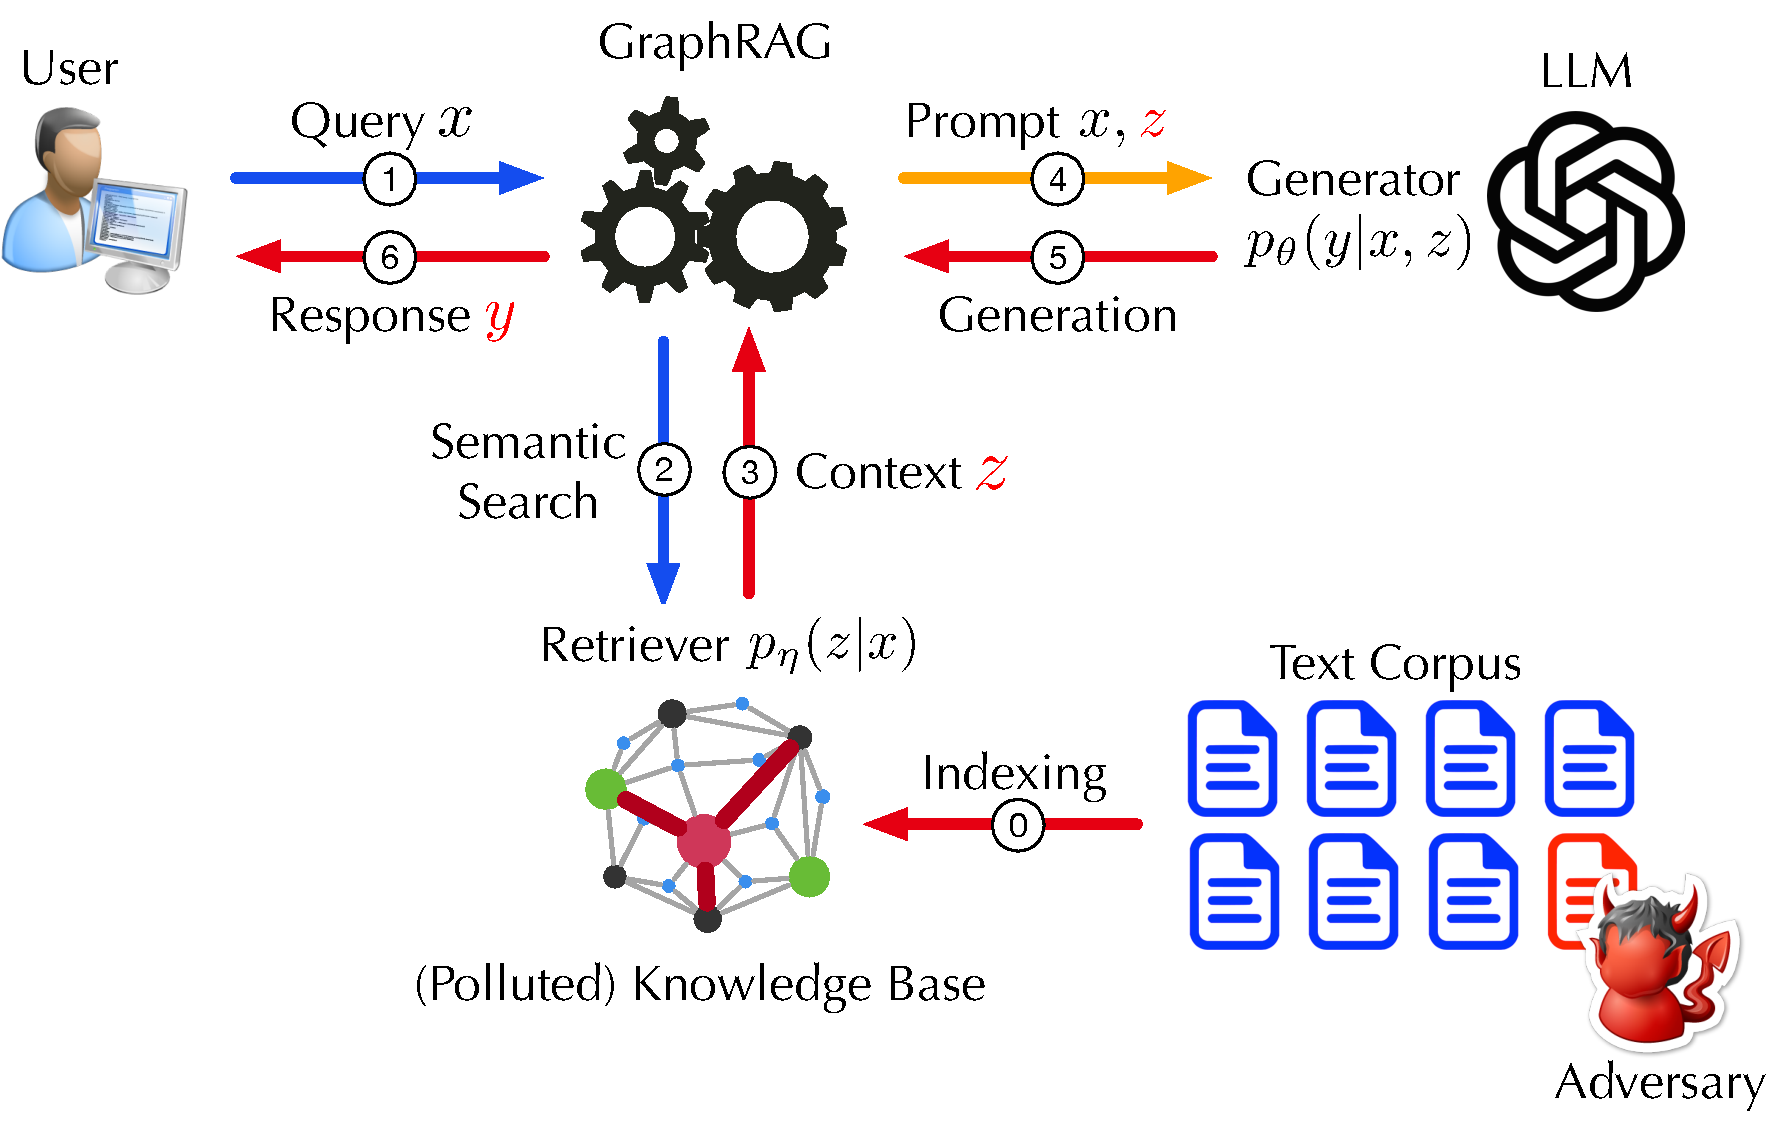
\includegraphics[width=1.\linewidth]{figs_false/gragpoison-attack.pdf}
    \caption{\small Poisoning attacks on \rag.}
    \label{fig:graphrag}
\end{figure}

Despite success across various domains, RAG-based models are often vulnerable to adversarial poisoning attacks, due to their fundamental reliance on external information to construct knowledge bases\mcite{thakur2021beir}. These attacks, where adversaries inject carefully crafted malicious content into knowledge bases to compromise LLM generation, have been extensively studied for conventional RAG frameworks\mcite{zouPoisonedRAGKnowledgeCorruption2024, dengPandoraJailbreakGPTs2024, xianVulnerabilityApplyingRetrievalAugmented2024, chengTrojanRAGRetrievalAugmentedGeneration2024}. In comparison, GraphRAG's security implications remain largely unexplored, raising key questions:

\vspace{2pt}
\noindent RQ1: Are existing RAG poisoning attacks still effective under GraphRAG?

\vspace{2pt}
\noindent RQ2: What unique vulnerabilities does GraphRAG have?

\vspace{2pt}
\noindent RQ3: What potential defensive measures exist?

\vspace{2pt}
{\bf Our Work.} To bridge this critical gap, we conduct a systematic study on \rag's vulnerability to poisoning attacks, revealing the following key insights:

\vspace{2pt}
\jc{\mct{i} \ul{
Existing RAG poisoning attacks are significantly less effective under GraphRAG.} Recall that \rag represents external knowledge as a multi-scale graph (\meg, entities, relations, and communities), and its graph-based indexing and retrieval pipeline often disrupts the intended effect of existing poisoning attacks: clean knowledge helps neutralize malicious content during indexing, while the graph structure effectively guides LLM reasoning and enables self-correction during inference. }


\jc{These design properties hinder existing attacks such as \prag, which rely on directly embedding misleading answers near target queries in the retrieval corpus. Our empirical findings (see \msec{sec:poisonedrag_on_graphrag}) show that such query-specific poisoning strategies suffer sharp performance degradation on GraphRAG compared to conventional RAG.} With the increasing number of target queries, existing poisoning attacks\mcite{zhong2023poisoning} that generate query-specific malicious content become less \yh{practical} due to the prohibitive computational cost, and more detectable due to the large corpus of poisoned text\mcite{wan2024dell, zhouTrustworthinessRetrievalAugmentedGeneration2024}.


\vspace{2pt}
\mct{ii} \ul{Meanwhile, the same features create new attack surfaces.} \yh{We present \attack, an effective and scalable black-box poisoning attack that exploits \rag's graph-based indexing and retrieval.} Intuitively, queries sharing relations in the knowledge graph can be attacked simultaneously. 
For instance, consider two queries \msf{How to mitigate the malware Stuxnet?} and \msf{How to detect the malware Stuxnet}, both relying on the relation \msf{Stuxnet uses DLL Injection}. Rather than attacking each query separately, injecting a false relation \msf{Stuxnet uses Process Hollowing} into the knowledge graph allows \attack to compromise both queries together, improving both attack effectiveness and scalability. 



Specifically, \attack assumes the adversary can only inject limited poisoning text into \rag's text corpora, without access to \rag's other components. At a high level, \attack crafts the poisoning text in three key steps. 
\mct{1} Relation selection -- It identifies critical relations shared across multiple target queries by analyzing their embedded relations;
\mct{2} Relation injection -- For each selected relation, it generates a false substitute (\meg, replacing \msf{Stuxnet uses DLL Injection} with \msf{Stuxnet uses Process Hollowing});
\mct{3} Relation enhancement -- It further strengthens each injected relation by adding supporting relations (\meg, \msf{Process Hallowing is detectable by Process Creation}). To resolve potential conflicts between poisoning and clean text, it employs an adversarial LLM to generate coherent narratives that naturally embed the malicious content.

Notably, while \attack exploits GraphRAG's graph-based indexing and retrieval, it differs fundamentally from conventional graph poisoning attacks\mcite{zhangDataPoisoningAttack2019, bhardwajPoisoningKnowledgeGraph2021, banerjeeStealthyTargetedData2021, xi2023security} in critical aspects. Graph poisoning attacks assume explicit knowledge about the graph structures, whereas \attack must infer these underlying structures through query analysis. Further, conventional attacks directly manipulate graph structures or node/edge features/embeddings, while \attack generates textual narratives that poison the source corpus. This creates a range of non-trivial challenges, including how to accurately infer the underlying graph structures and how to ensure the false information becomes indexed by \rag, preferentially retrieved for relevant queries, and ultimately trusted by the generator LLM, even potentially overriding conflicting legitimate information in the context.

Empirical evaluation across multiple GraphRAG variants (\meg, GraphRAG\mcite{graphrag} and LightRAG\mcite{guo2024lightrag}) and datasets (\meg, geographic, medical, and cyber-security) demonstrates that \attack substantially outperforms existing attacks in terms of attack effectiveness (achieving up to 98\%  success rate) and scalability (using 68\% less poisoning text).

\vspace{2pt}
\mct{iii} \ul{\textsc{GragPoison} is resilient to representative defenses.}
We examine various defenses against poisoning attacks, including leveraging LLMs' built-in knowledge to combat poisoning knowledge, paraphrasing incoming queries, and detecting false responses based on chain-of-thought (CoT) consistency. However, \attack remains effective against these countermeasures, suggesting that \attack exploits \rag's fundamental vulnerabilities and requires tailored defenses.


\vspace{2pt}
{\bf Our Contributions.} To the best of our knowledge, this represents the first work on exploring \rag's unique vulnerabilities to poisoning attacks. Our contributions are summarized as follows.
\begin{itemize}[leftmargin=*]
\item \jc{We show that existing poisoning attacks, though effective against conventional RAG, become significantly less effective on \rag due to its graph-based indexing and retrieval pipeline.}
\item We further reveal that these same features also create new vulnerabilities. We present \attack, a novel text-driven black-box attack tailored to \rag that crafts poisoning text targeting multiple queries simultaneously. Empirical evaluation shows that \attack significantly outperforms existing attacks in terms of both effectiveness and scalability on various graph-based RAG systems. 
\item We explore potential defensive measures against \attack and their fundamental limitations, identifying several promising directions for future research.
\end{itemize}

\yh{
This paper is structured as follows. We begin by reviewing the fundamentals of \rag and defining the threat model in \msec{sec:Preliminaries}. We then demonstrate the reduced effectiveness of conventional poisoning attacks on this new paradigm in \msec{sec:poisonedrag_on_graphrag}. We present \attack, a novel attack designed to exploit \rag's unique architecture in \msec{sec:GRAGPoison}, and empirically validate its effectiveness and scalability in \msec{sec:rq2}. Finally, we evaluate potential defensive measures in \msec{sec:rq3}.}
% \section{I

% \yh {Unlike traditional graph-based relation attacks \mcite{zhangDataPoisoningAttack2019, bhardwajPoisoningKnowledgeGraph2021,banerjeeStealthyTargetedData2021,xi2023security}, our method offers a significant advancement in LLM field. First, conventional feature-based attacks on text inputs become impractical and costly for LLMs with immense parameter spaces. Instead, we introduce a purely text-based attack specifically designed for \rag and LLMs. Furthermore, our embedding-free approach enables black-box execution and straightforward generalization across various LLM-based \rag systems.}




% Notably, while \prag exploits GraphRAG's graph-based indexing and retrieval mechanisms, it differs from conventional graph poisoning attacks in major aspects. First, graph poisoning attacks directly modify graph structures or node/edge features/embeddings\mcite{zhangDataPoisoningAttack2019, bhardwajPoisoningKnowledgeGraph2021, banerjeeStealthyTargetedData2021, xi2023security}, \rag's dynamic text-to-graph indexing creates a distinct vulnerability. Our attack, \prag, exploits this vulnerability by injecting malicious textual narratives into the source corpus. This strategy poisons the graph's semantic construction process, ensuring the false information becomes indexed by \rag, preferentially retrieved for relevant queries, and ultimately trusted by the generator LLM, even potentially overriding conflicting legitimate information in the context. This text-based manipulation, fundamentally different from traditional feature-based or structural attacks, facilitates black-box execution and generalizes across graph-based RAG systems.


% Long version
% \jc{While prior work on graph poisoning often involves directly modifying graph structures or perturbing node/edge embeddings~\cite{zhangDataPoisoningAttack2019, bhardwajPoisoningKnowledgeGraph2021, banerjeeStealthyTargetedData2021, xi2023security}, such approaches face challenges against \rag's dynamic, LLM-driven text-to-graph indexing process, which presents a distinct vulnerability. Our attack, \prag, is specifically designed for this context as a purely text-based method. Instead of directly altering the topology or embeddings within the graph, \prag operates by injecting malicious textual narratives into the source knowledge base. The core premise is to poison the input text itself, expecting \rag's indexing LLM to faithfully incorporate this adversarial content—representing false entities or relations—into its dynamically constructed knowledge graph. Furthermore, \prag aims not only for successful indexing but also for the resulting poisoned graph elements or narratives to be retrieved with high priority into the retrieval context window for targeted queries. Leveraging techniques like relation enhancement and narrative generation, the ultimate goal is to ensure that the generator LLM  trusts and utilizes the injected malicious information, even when potentially conflicting legitimate knowledge might also be present in the retrieved context. This focus on manipulating semantic construction via the textual source, influencing retrieval priority, and overriding conflicting context distinguishes \prag from traditional feature-based or structural graph attacks. Its text-based nature also facilitates black-box execution and straightforward generalization across various LLM-based \rag systems.}

% \jc{While Prior work on graph poisoning often involves directly modifying graph structures or perturbing node/edge embeddings \mcite{zhangDataPoisoningAttack2019, bhardwajPoisoningKnowledgeGraph2021,banerjeeStealthyTargetedData2021,xi2023security}. \rag's dynamic text-to-graph indexing presents a distinct vulnerability. Our attack, \prag, is specifically designed for this context as a purely text-based method. Instead of directly altering the topology of the graph or node/edge embeddings, \prag operates by injecting malicious textual narratives into the source knowledge base. This manipulation of semantic content poisons \rag's indexing phase, causing it to build a knowledge graph containing false information derived from the poisoned text. Targeting the graph's textual source to corrupt its semantic construction distinguishes \prag from traditional feature-based attacks on static graphs. Moreover, this text-based approach requires no direct manipulation or knowledge of internal embeddings, facilitating black-box execution and straightforward generalization across various LLM-based \rag systems.}

% \jc{While prior work on graph poisoning often involves directly modifying graph structures or perturbing node/edge features [cite relevant prior work], GraphRAG's dynamic text-to-graph construction presents a different vulnerability. Our attack, \prag , specifically targets this process. Instead of altering graph topology or features directly, \prag injects malicious textual narratives into the source knowledge base. This manipulation of semantic content poisons \rag's indexing phase, leading it to build a knowledge graph containing false information derived from the poisoned text. Targeting the graph's textual source to corrupt its semantic construction distinguishes \prag  from traditional feature-based attacks on static graphs.  }



